% ==============================================================
% ViT Token Economy — Beamer Presentation
% Generated from mte_results/  CSV data
% ==============================================================
\documentclass[aspectratio=169, 11pt]{beamer}

% ---------- theme & colours ----------
\usetheme{Madrid}
\usecolortheme{seahorse}
\setbeamertemplate{navigation symbols}{}
\setbeamertemplate{footline}[frame number]

% ---------- packages ----------
\usepackage{booktabs}
\usepackage{amsmath,amssymb}
\usepackage{graphicx}
\usepackage{tikz}
\usetikzlibrary{arrows.meta, positioning, calc, fit, shapes.geometric}
\usepackage{pgfplots}
\pgfplotsset{compat=1.18}
\usepackage{multirow}
\usepackage{xcolor}
\usepackage{hyperref}

% ---------- custom colours ----------
\definecolor{prunecolor}{RGB}{220,50,50}
\definecolor{mergecolor}{RGB}{50,120,200}
\definecolor{hybridcolor}{RGB}{120,50,180}
\definecolor{baselinecolor}{RGB}{0,150,80}

% ---------- title information ----------
\title[ViT Token Economy]{Training-Free Token Economy\\for Vision Transformers}
\subtitle{Hybrid Pruning + Merging on Pretrained ViT/DeiT Models}
\author{Chalhotra}
\institute{ViT Token Economy Project}
\date{\today}

% ==============================================================
\begin{document}

% ----------------------------------------------------------
% 1. TITLE
% ----------------------------------------------------------
\begin{frame}
\titlepage
\begin{center}
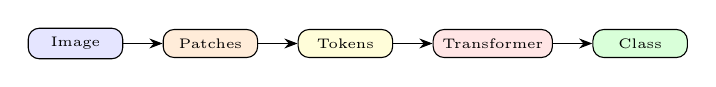
\begin{tikzpicture}[scale=0.55, every node/.style={font=\tiny}]
  \node[draw, rounded corners, fill=blue!10, minimum width=1.2cm] (img) {Image};
  \node[draw, rounded corners, fill=orange!15, right=0.5cm of img, minimum width=1.2cm] (patch) {Patches};
  \node[draw, rounded corners, fill=yellow!15, right=0.5cm of patch, minimum width=1.2cm] (tok) {Tokens};
  \node[draw, rounded corners, fill=red!10, right=0.5cm of tok, minimum width=1.4cm] (trans) {Transformer};
  \node[draw, rounded corners, fill=green!15, right=0.5cm of trans, minimum width=1.2cm] (cls) {Class};
  \draw[-{Stealth}] (img) -- (patch);
  \draw[-{Stealth}] (patch) -- (tok);
  \draw[-{Stealth}] (tok) -- (trans);
  \draw[-{Stealth}] (trans) -- (cls);
\end{tikzpicture}
\end{center}
\end{frame}

% ----------------------------------------------------------
% 2. MOTIVATION
% ----------------------------------------------------------
\begin{frame}{Motivation}
\begin{columns}[T]
\column{0.55\textwidth}
\begin{itemize}
  \item Vision Transformers achieve \textbf{strong performance} on image classification
  \item But they are \textbf{computationally expensive}
  \item An image is split into many patches $\rightarrow$ \textbf{many tokens}
  \item Self-attention cost grows \textbf{quadratically}
\end{itemize}

\vspace{0.4cm}
\textbf{Example — ViT-B/16}
\begin{itemize}
  \item $224 \times 224$ image $\rightarrow$ $14 \times 14 = \mathbf{196}$ tokens
  \item Baseline GFLOPs: \textbf{16.87}
  \item Baseline Top-1 Accuracy: \textbf{95.52\%}
\end{itemize}

\column{0.42\textwidth}
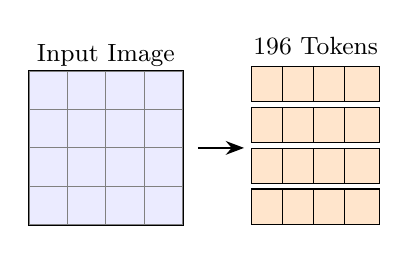
\begin{tikzpicture}[scale=0.65]
  % image
  \draw[thick, fill=blue!8] (0,0) rectangle (3,3);
  \node at (1.5,3.3) {\small Input Image};
  % grid
  \foreach \x in {0,0.75,...,2.25}
    \foreach \y in {0,0.75,...,2.25}
      \draw[gray] (\x,\y) rectangle (\x+0.75,\y+0.75);
  % arrow
  \draw[-{Stealth}, thick] (3.3,1.5) -- (4.2,1.5);
  % tokens
  \foreach \i in {0,...,3} {
    \foreach \j in {0,...,3} {
      \node[draw, fill=orange!20, minimum size=0.45cm, inner sep=0pt,
            font=\tiny] at (4.7+\j*0.6, 0.35+\i*0.8) {};
    }
  }
  \node at (5.6,3.5) {\small 196 Tokens};
\end{tikzpicture}
\end{columns}
\end{frame}

% ----------------------------------------------------------
% 3. PROBLEM STATEMENT
% ----------------------------------------------------------
\begin{frame}{Problem Statement}
\begin{columns}[T]
\column{0.52\textwidth}
Self-attention computes interactions between \textbf{all} token pairs:
\[
  \mathrm{Attention}(Q,K,V)
  = \mathrm{Softmax}\!\Bigl(\frac{QK^{\!\top}}{\sqrt{d}}\Bigr)V
\]

\textbf{Complexity:} $\mathcal{O}(N^{2})$ where $N$ = number of tokens.

\vspace{0.3cm}
\textbf{Key Observation:}
\begin{itemize}
  \item Many tokens correspond to \textbf{redundant background} regions
  \item Not all tokens contribute equally to the final prediction
\end{itemize}

\vspace{0.3cm}
\textbf{Goal:} Reduce token count $N$ while \textbf{preserving accuracy}.

\column{0.45\textwidth}
% --- Diagram: fully connected attention graph ---
\begin{center}
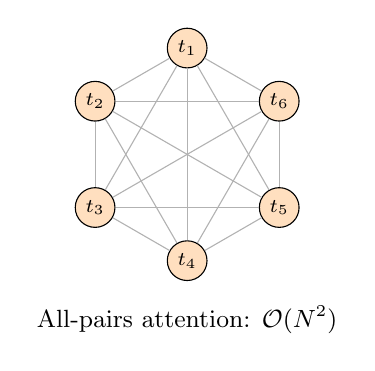
\begin{tikzpicture}[scale=0.75]
  \def\n{6}
  \foreach \i in {1,...,\n} {
    \pgfmathsetmacro{\angle}{90 + (\i-1)*360/\n}
    \node[circle, draw, fill=orange!25, inner sep=2pt,
          minimum size=0.5cm, font=\scriptsize]
          (t\i) at (\angle:1.8cm) {$t_{\i}$};
  }
  \foreach \i in {1,...,\n} {
    \foreach \j in {\i,...,\n} {
      \draw[gray!60, thin] (t\i) -- (t\j);
    }
  }
  \node[below=0.3cm, font=\small] at (0,-2) {All-pairs attention: $\mathcal{O}(N^2)$};
\end{tikzpicture}
\end{center}
\end{columns}
\end{frame}

% ----------------------------------------------------------
% 4. VISION TRANSFORMER OVERVIEW
% ----------------------------------------------------------
\begin{frame}{Vision Transformer Overview}
\begin{center}
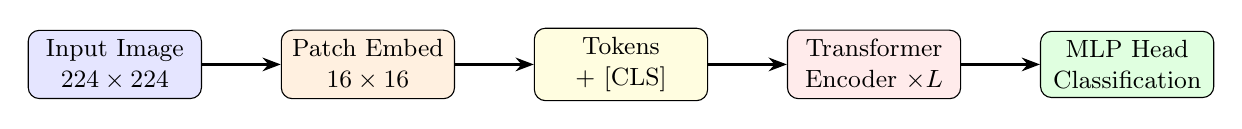
\begin{tikzpicture}[
    node distance=0.7cm and 1.0cm,
    box/.style={draw, rounded corners, minimum height=0.8cm,
                minimum width=2.2cm, font=\small, align=center},
    arr/.style={-{Stealth}, thick}
  ]
  \node[box, fill=blue!10]   (img)   {Input Image\\$224\times224$};
  \node[box, fill=orange!12, right=of img]   (patch) {Patch Embed\\$16\times16$};
  \node[box, fill=yellow!12, right=of patch] (tok)   {Tokens\\+ [CLS]};
  \node[box, fill=red!8,     right=of tok]   (enc)   {Transformer\\Encoder $\times L$};
  \node[box, fill=green!12,  right=of enc]   (head)  {MLP Head\\Classification};
  \draw[arr] (img)   -- (patch);
  \draw[arr] (patch) -- (tok);
  \draw[arr] (tok)   -- (enc);
  \draw[arr] (enc)   -- (head);
\end{tikzpicture}
\end{center}

\vspace{0.3cm}
\textbf{Key Components:}
\begin{itemize}
  \item \textbf{Patch Embedding}: Split image into $16\times16$ non-overlapping patches, linearly project
  \item \textbf{Class Token [CLS]}: Learnable token prepended; aggregates global information
  \item \textbf{Self-Attention Layers}: Multi-head attention + FFN at every layer
  \item \textbf{Classification Head}: MLP on [CLS] token output
\end{itemize}
\end{frame}

% ----------------------------------------------------------
% 5. EXISTING TOKEN REDUCTION METHODS
% ----------------------------------------------------------
\begin{frame}{Existing Token Reduction Methods}
\begin{table}[h]
\centering
\small
\begin{tabular}{@{}llll@{}}
\toprule
\textbf{Category} & \textbf{Method} & \textbf{Mechanism} & \textbf{Training?} \\
\midrule
\multirow{2}{*}{Token Pruning}
  & DynamicViT & Learned pruning decisions     & Yes \\
  & EViT       & CLS-attention top-K + fuse rest & No  \\
\midrule
\multirow{1}{*}{Token Merging}
  & ToMe       & Bipartite soft-matching merge  & No  \\
\midrule
\multirow{1}{*}{Hybrid}
  & \textbf{EViT + ToMe} & Prune then merge      & \textbf{No}  \\
\bottomrule
\end{tabular}
\end{table}

\vspace{0.3cm}
\textbf{Important:}
\begin{itemize}
  \item Some approaches (\textit{e.g.}, DynamicViT) require \textbf{additional training} or fine-tuning
  \item Training-free methods are preferable for deploying with \textbf{off-the-shelf} pretrained models
\end{itemize}
\end{frame}

% ----------------------------------------------------------
% 6. RESEARCH GAP
% ----------------------------------------------------------
\begin{frame}{Research Gap}
\begin{itemize}
  \item Many token reduction methods \textbf{require training or retraining}
  \item Some approaches \textbf{modify the training pipeline}, making deployment harder
  \item Efficient approaches for \textbf{off-the-shelf pretrained models} are limited
  \item \textbf{Hybrid} pruning + merging strategies remain under-explored in a training-free setting
\end{itemize}

\vspace{0.6cm}
\begin{center}
\fcolorbox{hybridcolor}{hybridcolor!8}{%
  \parbox{0.75\textwidth}{\centering
    \textbf{Our Idea:}
    Explore \textbf{training-free} token reduction\\
    combining pruning and merging on pretrained ViT/DeiT models.
  }
}
\end{center}
\end{frame}

% ----------------------------------------------------------
% 7. OUR CONTRIBUTIONS
% ----------------------------------------------------------
\begin{frame}{Our Contributions}
\begin{enumerate}
  \item \textbf{Training-free token reduction framework}\\
        Works directly on pretrained ViT/DeiT — no fine-tuning needed
  \item \textbf{Hybrid pruning + merging strategy (EViT + ToMe)}\\
        Two-stage pipeline combining EViT fusion and ToMe bipartite matching
  \item \textbf{Proportional attention} to stabilise merging\\
        Attention weights scaled by the number of merged tokens
  \item \textbf{Comprehensive evaluation} across six models and four keep rates\\
        Measuring accuracy, GFLOPs, throughput, and latency on ImageNet-100
  \item \textbf{Multiple efficiency profiles}\\
        Balanced, pruning-heavy, and merging-heavy configurations
\end{enumerate}
\end{frame}

% ----------------------------------------------------------
% 8. HYBRID TOKEN REDUCTION METHOD
% ----------------------------------------------------------
\begin{frame}{Hybrid Token Reduction Pipeline}
\begin{center}
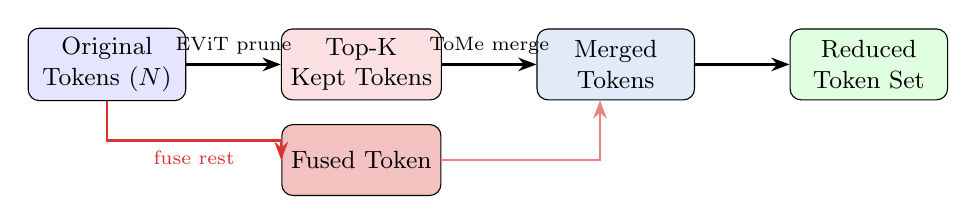
\begin{tikzpicture}[
    node distance=0.4cm and 0.6cm,
    stage/.style={draw, rounded corners, minimum height=0.9cm,
                  minimum width=2.0cm, font=\small, align=center},
    arr/.style={-{Stealth}, thick},
    lbl/.style={font=\scriptsize, midway, above}
  ]
  % Stage 1
  \node[stage, fill=blue!10] (orig) {Original\\Tokens ($N$)};

  % Stage 2 — EViT pruning
  \node[stage, fill=prunecolor!15, right=1.2cm of orig] (prune) {Top-K\\Kept Tokens};
  \node[stage, fill=prunecolor!30, below=0.3cm of prune, minimum width=1.6cm]
        (fuse) {Fused Token};

  % Stage 3 — ToMe merging
  \node[stage, fill=mergecolor!15, right=1.2cm of prune] (merged) {Merged\\Tokens};

  % Output
  \node[stage, fill=green!12, right=1.2cm of merged] (out) {Reduced\\Token Set};

  % Arrows
  \draw[arr] (orig) -- node[lbl]{EViT prune} (prune);
  \draw[arr, prunecolor] (orig.south) -- ++(0,-0.5) -| (fuse.west)
        node[pos=0.25, below, font=\scriptsize]{fuse rest};
  \draw[arr] (prune) -- node[lbl]{ToMe merge} (merged);
  \draw[arr, prunecolor!60] (fuse.east) -| ($(merged.south)-(0.2,0)$);
  \draw[arr] (merged) -- (out);
\end{tikzpicture}
\end{center}

\vspace{0.4cm}
\textbf{Stage Details:}
\begin{enumerate}
  \item \textbf{EViT Pruning}: Rank tokens by CLS-attention; keep top-K; fuse the rest into one token
  \item \textbf{ToMe Merging}: Partition tokens into two groups (even/odd index);
        bipartite soft-matching merges the most similar pairs
  \item Output: a \textbf{reduced token set} fed to subsequent layers
\end{enumerate}
\end{frame}

% ----------------------------------------------------------
% 9. PROPORTIONAL ATTENTION
% ----------------------------------------------------------
\begin{frame}{Proportional Attention}
\textbf{Problem:} After merging, each token may represent a \emph{different} number of original tokens.

\vspace{0.3cm}
\textbf{Solution — Proportional Attention:}
\[
  \widetilde{A}_{ij}
  = \frac{s_j \cdot \exp\!\bigl(\tfrac{q_i \cdot k_j}{\sqrt{d}}\bigr)}
         {\sum_{l} s_l \cdot \exp\!\bigl(\tfrac{q_i \cdot k_l}{\sqrt{d}}\bigr)}
\]
where $s_j$ is the \textbf{size} (number of original tokens) represented by token $j$.

\vspace{0.3cm}
\textbf{Benefits:}
\begin{itemize}
  \item Maintains \textbf{information balance} — larger merged groups receive proportionally more attention
  \item Prevents merged tokens from \textbf{losing importance} despite representing many patches
  \item Fully \textbf{training-free}: only modifies the softmax normalisation at inference
\end{itemize}
\end{frame}

% ----------------------------------------------------------
% 10. EXPERIMENTAL SETUP
% ----------------------------------------------------------
\begin{frame}{Experimental Setup}
\begin{columns}[T]
\column{0.48\textwidth}
\textbf{Models (pretrained, timm):}
\begin{itemize}
  \item ViT-Tiny/16 \quad(5.54\,M params)
  \item ViT-Small/16 \quad(21.70\,M)
  \item ViT-Base/16 \quad(85.88\,M)
  \item DeiT-Tiny/16 \quad(5.54\,M)
  \item DeiT-Small/16 \quad(21.70\,M)
  \item DeiT-Base/16 \quad(85.88\,M)
\end{itemize}

\column{0.48\textwidth}
\textbf{Dataset:}
\begin{itemize}
  \item ImageNet-100 (100-class subset)
\end{itemize}

\vspace{0.3cm}
\textbf{Metrics:}
\begin{itemize}
  \item Top-1 Accuracy (\%)
  \item GFLOPs
  \item Throughput (images/sec)
  \item Latency (ms/image)
\end{itemize}
\end{columns}

\vspace{0.4cm}
\begin{center}
\fcolorbox{baselinecolor}{baselinecolor!8}{%
  \parbox{0.7\textwidth}{\centering
    \textbf{No training or fine-tuning performed.}\\
    All evaluations are \textbf{inference-time only} modifications.
  }
}
\end{center}
\end{frame}

% ----------------------------------------------------------
% 11. RESULTS — Accuracy vs GFLOPs
% ----------------------------------------------------------
\begin{frame}{Results — Accuracy vs.\ GFLOPs}
\begin{center}
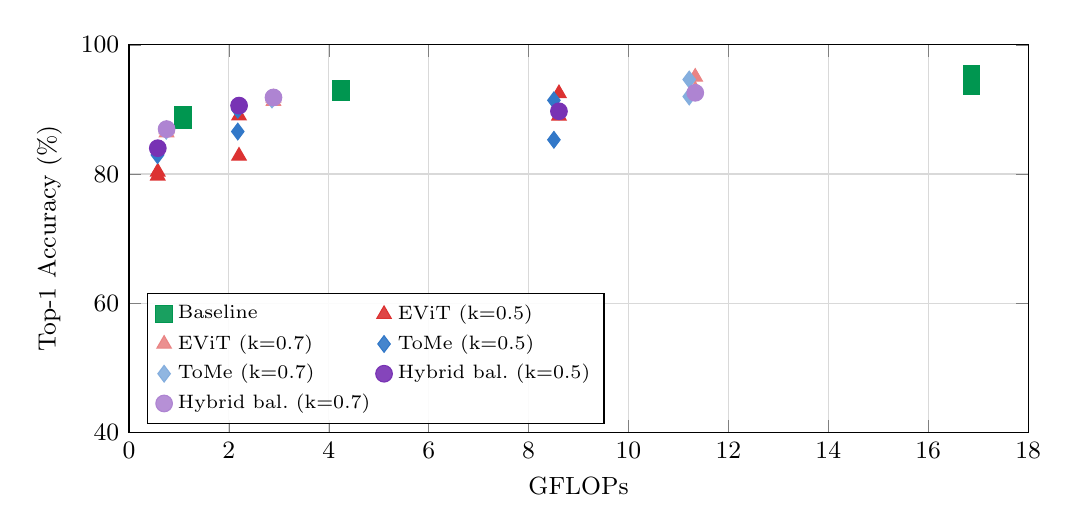
\begin{tikzpicture}
\begin{axis}[
    width=13cm, height=6.5cm,
    xlabel={GFLOPs}, ylabel={Top-1 Accuracy (\%)},
    xmin=0, xmax=18, ymin=40, ymax=100,
    grid=major, grid style={gray!30},
    legend style={at={(0.02,0.02)}, anchor=south west, font=\scriptsize,
                  cells={anchor=west}, fill=white, fill opacity=0.9,
                  draw opacity=1, text opacity=1},
    legend columns=2,
    tick label style={font=\small},
    label style={font=\small},
]

% --- Baseline ---
\addplot[only marks, mark=square*, mark size=3pt, baselinecolor]
  coordinates {
    (1.079,88.42) (1.079,89.22)
    (4.250,92.62) (4.250,93.18)
    (16.867,93.64) (16.867,95.52)
  };
\addlegendentry{Baseline}

% --- EViT (keep=0.5) ---
\addplot[only marks, mark=triangle*, mark size=3pt, prunecolor]
  coordinates {
    (0.576,80.34) (0.576,79.72)
    (2.203,89.02) (2.203,82.80)
    (8.608,89.00) (8.608,92.48)
  };
\addlegendentry{EViT (k=0.5)}

% --- EViT (keep=0.7) ---
\addplot[only marks, mark=triangle*, mark size=3pt, prunecolor!60]
  coordinates {
    (0.752,86.42) (0.752,86.92)
    (2.892,91.80) (2.892,91.28)
    (11.336,93.06) (11.336,95.04)
  };
\addlegendentry{EViT (k=0.7)}

% --- ToMe (keep=0.5) ---
\addplot[only marks, mark=diamond*, mark size=3pt, mergecolor]
  coordinates {
    (0.571,82.92) (0.571,83.06)
    (2.178,89.96) (2.178,86.58)
    (8.507,85.30) (8.507,91.42)
  };
\addlegendentry{ToMe (k=0.5)}

% --- ToMe (keep=0.7) ---
\addplot[only marks, mark=diamond*, mark size=3pt, mergecolor!60]
  coordinates {
    (0.746,86.70) (0.746,86.86)
    (2.863,91.54) (2.863,91.68)
    (11.216,92.00) (11.216,94.64)
  };
\addlegendentry{ToMe (k=0.7)}

% --- Hybrid balanced (keep=0.5) ---
\addplot[only marks, mark=*, mark size=3pt, hybridcolor]
  coordinates {
    (0.577,84.00)
    (2.204,90.60)
    (8.608,89.72)
  };
\addlegendentry{Hybrid bal.\ (k=0.5)}

% --- Hybrid balanced (keep=0.7) ---
\addplot[only marks, mark=*, mark size=3pt, hybridcolor!60]
  coordinates {
    (0.753,86.96)
    (2.893,91.86)
    (11.337,92.58)
  };
\addlegendentry{Hybrid bal.\ (k=0.7)}

\end{axis}
\end{tikzpicture}
\end{center}
\vspace{-0.2cm}
{\scriptsize DeiT-Tiny, DeiT-Small, DeiT-Base shown. ViT variants follow similar trends.}
\end{frame}

% ----------------------------------------------------------
% 11b. RESULTS — Table
% ----------------------------------------------------------
\begin{frame}{Results — Numerical Comparison (ViT-Base/16)}
\begin{table}[h]
\centering
\small
\begin{tabular}{@{}llrrr@{}}
\toprule
\textbf{Method} & \textbf{Keep Rate} & \textbf{Acc@1 (\%)} & \textbf{GFLOPs} & \textbf{Throughput} \\
\midrule
Baseline        & 1.00 & 95.52 & 16.87 & 78.6 \\
\midrule
EViT            & 0.90 & 95.54 & 14.99 & 86.4 \\
EViT            & 0.70 & 95.04 & 11.34 & 113.4 \\
EViT            & 0.50 & 92.48 &  8.61 & 149.3 \\
\midrule
ToMe            & 0.90 & 95.30 & 14.86 & 97.1 \\
ToMe            & 0.70 & 94.64 & 11.22 & 135.8 \\
ToMe            & 0.50 & 91.42 &  8.51 & 166.1 \\
\midrule
Hybrid (bal.)   & 0.90 & 93.56 & 15.01 & 98.1 \\
Hybrid (bal.)   & 0.70 & 92.58 & 11.34 & 131.1 \\
Hybrid (bal.)   & 0.50 & 89.72 &  8.61 & 169.9 \\
\bottomrule
\end{tabular}
\end{table}
\vspace{0.2cm}
\textbf{Key Takeaway:} Token reduction methods significantly reduce GFLOPs and increase throughput with modest accuracy trade-offs on pretrained ViT-Base/16.
\end{frame}

% ----------------------------------------------------------
% 11c. RESULTS — Hybrid Profiles
% ----------------------------------------------------------
\begin{frame}{Results — Hybrid Efficiency Profiles (DeiT-Small/16)}
\begin{table}[h]
\centering
\small
\begin{tabular}{@{}llrrrr@{}}
\toprule
\textbf{Budget} & \textbf{Profile} & \textbf{Acc@1} & \textbf{GFLOPs} & \textbf{Acc/GFLOP} & \textbf{Tput} \\
\midrule
0.50 & Balanced       & 90.60 & 2.20 & 41.12 & 614.1 \\
0.50 & Pruning-heavy  & 90.40 & 2.22 & 40.74 & 614.3 \\
0.50 & Merging-heavy  & 90.26 & 2.22 & 40.67 & 621.2 \\
\midrule
0.70 & Merging-heavy  & 92.06 & 2.89 & 31.82 & 463.5 \\
0.70 & Pruning-heavy  & 91.96 & 2.89 & 31.79 & 458.0 \\
0.70 & Balanced       & 91.86 & 2.89 & 31.75 & 462.0 \\
\midrule
0.90 & Balanced       & 92.30 & 3.82 & 24.14 & 341.3 \\
0.90 & Merging-heavy  & 92.28 & 3.82 & 24.14 & 341.2 \\
0.90 & Pruning-heavy  & 92.26 & 3.83 & 24.06 & 343.2 \\
\bottomrule
\end{tabular}
\end{table}
\vspace{0.2cm}
All three profiles achieve comparable accuracy; the \textbf{balanced} profile slightly leads at 0.50 and 0.90 budgets.
\end{frame}

% ----------------------------------------------------------
% 12. OBSERVATIONS
% ----------------------------------------------------------
\begin{frame}{Observations}
\begin{enumerate}
  \item \textbf{Aggressive pruning hurts accuracy significantly}\\
        At keep rate 0.25, EViT drops to 61.00\% on ViT-Base (vs.\ 95.52\% baseline)
  \item \textbf{Merging degrades more gracefully than pruning}\\
        ToMe at 0.50 retains 91.42\% on ViT-Base vs.\ 92.48\% for EViT
  \item \textbf{Proportional attention stabilises merged token performance}\\
        Prevents information loss in deep layers after repeated merging
  \item \textbf{Hybrid merging-heavy profile excels at low budgets}\\
        At budget 0.25, merging-heavy achieves 74.98\% vs.\ 67.62\% balanced on DeiT-Tiny
  \item \textbf{EViT alone at keep rate 0.90 matches or exceeds the baseline}\\
        ViT-Base: 95.54\% at 14.99 GFLOPs vs.\ 95.52\% at 16.87 GFLOPs
  \item \textbf{Throughput improvements are substantial}\\
        Up to $\sim$2$\times$ speedup at keep rate 0.50 across all model sizes
\end{enumerate}
\end{frame}

% ----------------------------------------------------------
% 13. FUTURE WORK
% ----------------------------------------------------------
\begin{frame}{Future Work}
\begin{itemize}
  \item \textbf{Adaptive token reduction}\\
        Layer-wise or input-dependent keep rates instead of fixed schedules
  \item \textbf{Learnable pruning strategies}\\
        Light-weight gating modules trained with minimal overhead
  \item \textbf{Hardware-aware optimisation}\\
        Tune reduction schedules for specific GPU/accelerator architectures
  \item \textbf{Extension to dense prediction tasks}\\
        Apply token economy to object detection and segmentation backbones
\end{itemize}
\end{frame}

% ----------------------------------------------------------
% 14. REFERENCES
% ----------------------------------------------------------
\begin{frame}{References}
\small
\begin{enumerate}
  \item Dosovitskiy \textit{et al.}, ``An Image is Worth 16x16 Words: Transformers for Image Recognition at Scale,'' \textit{ICLR}, 2021.
  \item Touvron \textit{et al.}, ``Training data-efficient image transformers \& distillation through attention,'' \textit{ICML}, 2021.
  \item Rao \textit{et al.}, ``DynamicViT: Efficient Vision Transformers with Dynamic Token Sparsification,'' \textit{NeurIPS}, 2021.
  \item Liang \textit{et al.}, ``Not All Patches are What You Need: Expediting Vision Transformers via Token Reorganizations,'' (EViT) \textit{ICLR}, 2022.
  \item Bolya \textit{et al.}, ``Token Merging: Your ViT But Faster,'' (ToMe) \textit{ICLR}, 2023.
  \item Bolya \textit{et al.}, ``Token Merging for Fast Stable Diffusion,'' \textit{CVPR Workshop}, 2023.
\end{enumerate}
\end{frame}

% ----------------------------------------------------------
% THANK YOU
% ----------------------------------------------------------
\begin{frame}
\begin{center}
  {\Huge Thank You!}

  \vspace{1cm}
  {\large Questions?}

  \vspace{0.5cm}
  \url{https://github.com/Chalhotra/ViT-Token-Economy}
\end{center}
\end{frame}

\end{document}
